%!TEX ROOT=geometria1.tex

\section{Matrici}%
\label{sec:matrici}

\subsection{Definizioni}%
\label{sub:definizioni_e_teoremi}

\begin{Def}{Matrice}
  Siano $m,n\in\mathbb{N}_0$. Una matrice di $m$ righe e $n$ colonne ad elementi reali è
  una tabella del tipo
  \begin{equation*}
    A =
    \begin{pmatrix}[1]
      a_{1,1} & a_{1,2} & \cdots & a_{1,n} \\
      a_{2,1} & a_{2,2} & \cdots & _{2,n} \\
      \vdots  & \vdots  & \ddots & \vdots  \\
      a_{m,1} & a_{m,2} & \cdots & a_{m,n}
    \end{pmatrix}
  \end{equation*}
  con $a_{ij}\in\mathbb{R}$ e $1\leq i\leq m$ e $1\leq j\leq n$.
\end{Def}

\begin{Def}{Ordine}
  Si dice \textbf{ordine} di una matrice si intendono le sue dimensioni, in questo caso
  $A$ è di ordine $m\times n$.
\end{Def}

Dato che una matrice contiene elementi reali, l'insieme di queste matrici viene definito
\begin{equation*}
  \mathbb{R}^{m,n}\bydef \{\text{Matrici reali di ordine }m\times n\}
\end{equation*}
Spesso una matrice viene definita anche in maniera più stringata
\begin{equation*}
  A = (a_{ij})\in\mathbb{R}^{m,n}
\end{equation*}

\begin{Def}{Matrice quadrata}
  Una matrice si dice quadrata quando $m=n$.
\end{Def}

\begin{Def}{Matrice identità}
  La matrice identità (o matrice unità) si definisce
  \begin{equation*}
    I\in\mathbb{R}^{m,n}\bydef
    \begin{pmatrix}
      1 & 0 & \cdots & 0\\
      0 & 1 & 0 & \vdots\\
      \vdots & 0 & 1 & 0\\
      0 & \cdots & 0 & 1
    \end{pmatrix}
  \end{equation*}
  Ovvero quella matrice la cui diagonale principale è formata da $1$ e tutto il resto da
  $0$. Formalmente
  \begin{equation*}
    a_{ij} =
    \begin{cases}
      0, &\text{ se }i\neq j\\
      1, &\text{ se }i=j
    \end{cases}
  \end{equation*}
\end{Def}

\begin{Def}{Diagonale principale}
  La diagonale principale di una matrice è quella descritta dagli elementi $a_{ii}$. Qui
  è colorata in blu.
  \begin{center}
    \begin{tikzpicture}[baseline=(A.center), scale=0.5]
      \tikzset{node style ge/.style={circle}}
      \tikzset{bar/.style = {opacity=.3,line width=4 mm,line cap=round,color=#1}}
      \tikzset{plus/.style = {above left,,opacity=1,circle,fill=#1!50}}
      \tikzset{minus/.style = {below left,,opacity=1,circle,fill=#1!50}}

      \matrix (A) [matrix of math nodes, nodes = {node style ge}, left delimiter = (,
      right delimiter = ),column sep=0 mm]
      {a_{11} & a_{12} & a_{13}\\
        a_{21} & a_{22} & a_{23}\\
        a_{31} & a_{32} & a_{33}\\
      };

      \draw [bar=blue] (A-1-1.north west) to (A-3-3.south east);
    \end{tikzpicture}
  \end{center}
\end{Def}

\begin{Def}{Matrice nulla}
  Per matrice nulla si intende
  \begin{equation*}
    O\in\mathbb{R}^{m,n}\bydef
    \begin{pmatrix}[1]
      0&\cdots&0\\
      \vdots & \ddots & \vdots\\
      0 & \cdots & 0
    \end{pmatrix}
  \end{equation*}
  Ovvero è la matrice tale che
  \begin{equation*}
    \forall i,j \quad a_{ij}=0
  \end{equation*}
\end{Def}

\begin{Def}{Matrice riga}
  Per matrice riga si intende quella che ha $m=1$, ovvero
  \begin{equation*}
    A =
    \begin{pmatrix}
      a_{11} & \cdots & a_{1n}
    \end{pmatrix}
    \in\mathbb{R}^{1,n}
  \end{equation*}
\end{Def}

\begin{Def}{Matrice colonna}
  Per matrice colonna si intende quella che ha $n=1$, ovvero
  \begin{equation*}
    A =
    \begin{pmatrix}
      a_{11}\\
      \vdots\\
      a_{m1}
    \end{pmatrix}
    \in\mathbb{R}^{m,1}
  \end{equation*}
\end{Def}

\begin{Def}{Matrice simmetrica}
  Sia $A\in\mathbb{R}^{n,n}$. $A$ è simmetrica se $\transp A = A$. Ovvero se
  \begin{equation*}
    a_{ij} = a_{ji}\quad\forall i,j=1,\ldots,n
  \end{equation*}
\end{Def}

\begin{Def}{Matrice antisimmetrica}
  Sia $A\in\mathbb{R}^{n,n}$. $A$ è antisimmetrica se $\transp A = -A$. Ovvero se
  \begin{equation*}
    a_{ij} = -a_{ji}\quad \forall i,j=1,\ldots,n
  \end{equation*}
\end{Def}

\begin{Def}{Matrice invertibile}\label{def:matrice_inversa}
  Sia $A$ una matrice quadrata. $A$ è in vertibile o non singolare se
  \begin{equation*}
    \exists X\in\mathbb{R}^{n,n}\suchthat AX = XA = I
  \end{equation*}
  Si noti che si indica $X = A^{-1}$.
\end{Def}

\begin{Thm}{Unicità dell'inversa}
  Se $A\in\mathbb{R}^{n,n}$ è invertibile allora la matrice inversa è unica.
\end{Thm}

\begin{proof}
  Sopponiamo per assurdo che $\exists X,X'\in\mathbb{R}^{n,n}$ con $X\neq X'$ tali che
  \begin{equation*}
    AX'=X'A=AX=XA=I
  \end{equation*}
  Allora
  \begin{equation*}
    X'=IX' = (XA)X' = X(AX') = XI = X
  \end{equation*}
\end{proof}

\begin{SubDef}{Proprietà della matrice inversa}
  La matrice inversa gode di alcune proprietà:
  \begin{enumerate}
    \item $(AB)^{-1} = B^{-1}A^{-1}\quad\forall A,B\in\mathbb{R}^{n,n}$
      \begin{proof}
        Dobbiamo dimostrare $B^{-1}A^{-1}={(AB)}^{-1}\iff
          AB(A^{-1}B^{-1})=(A^{-1}B^{-1})AB=I$ per la~\autoref{def:matrice_inversa}.
          Quindi
          \begin{equation*}
            B^{-1}A^{-1}(AB) = B^{-1}(A^{-1}A)B = B^{-1}B = I
          \end{equation*}
          e
          \begin{equation*}
            AB(A^{-1}B^{-1}) = A(BB^{-1})A^{-1} = AA^{-1} = I
          \end{equation*}
      \end{proof}
    \item ${(A^{-1})}^{-1}\quad\forall A\in\mathbb{R}^{n,n}$
      \begin{proof}
        Per~\autoref{def:matrice_inversa}
        \begin{equation*}
          A^{-1}A = AA^{-1} = I
        \end{equation*}
      \end{proof}
  \end{enumerate}
\end{SubDef}

\begin{SubDef}{Gruppo lineare}
  Si definisce un gruppo lineare l'insieme
  \begin{equation*}
    GL(n,\mathbb{R})\bydef \left\{ A\in\mathbb{R}^{n,n}\Setsuchthat A\text{ è
    invertibile} \right\}
  \end{equation*}
  assieme al prodotto.
\end{SubDef}

\begin{Def}{Matrice diagonale}
  Sia $A\in\mathbb{R}^{n,n} = (a_{ij})$. Si dice diagonale se
  \begin{equation*}
    \forall i,j = 1,\ldots,n\suchthat i\neq j\quad a_{ij} = 0
  \end{equation*}
  Ovvero
  \begin{equation*}
    \mqty(\dmat[0]{a_{11}, a_{22}, \ddots, a_{nn}})
  \end{equation*}
\end{Def}

\subsection{Operazioni}%
\label{sub:operazioni}

\begin{Def}{Uguaglianza}
  Due matrici $A=(a_{ij})\in\mathbb{R}^{m,n}$ e $B=(b_{ij})\in\mathbb{R}^{p,q}$ si dicono
  uguali se
  \begin{enumerate}
    \item $A$ e $B$ appartengono allo stesso insieme $\mathbb{R}^{m,n}$, ovvero $m=p$ e
      $n=q$
    \item $a_{ij} = b_{ij},\quad\forall i:\,1\leq i\leq m \quad\forall j:\,1\leq j\leq n$
  \end{enumerate}
\end{Def}

\begin{Def}{Somma}\label{def:matrice_somma}
  La somma tra matrici è solo definita se le due matrici appartengono allo stesso
  insieme.\\
  Siano $A=(a_{ij})\in\mathbb{R}^{m,n}$ e $B=(b_{ij})\in\mathbb{R}^{m,n}$ due matrici.
  La loro somma $A+B$ è
  \begin{equation*}
    A+B\bydef (a_{ij}+b_{ij})
  \end{equation*}
  Si definisce quindi anche l'operatore somma nel seguente modo
  \begin{align*}
    +:&\;\mathbb{R}^{m,n}\times\mathbb{R}^{m,n}\rightarrow\mathbb{R}^{m,n}\\
      & (A,B)\mapsto A+B
  \end{align*}
\end{Def}

\begin{SubDef}{Proprietà della somma tra matrici}
  Per la somma tra matrici valgono le seguenti proprietà:
  \begin{enumerate}
    \item Commutativa: $A+B = B+A\quad\forall A,B\in\mathbb{R}^{m,n}$
    \item Associativa: $A+(B+C) = (A+B)+C\quad\forall A,B,C\in\mathbb{R}^{m,n}$
    \item Esistenza dell'elemento neutro: $O+A = A+O\quad\forall A\in\mathbb{R}^{m,n}$
    \item Esistenza dell'opposto: $A+(-A) = 0\quad\forall A\in\mathbb{R}^{m,n}$
  \end{enumerate}
\end{SubDef}

\begin{Def}{Prodotto tra matrice e scalare}\label{def:matrice_prodotto_scalare}
  Si definisce il prodotto tra $\lambda\in\mathbb{R}$ e $A=(a_{ij})\in\mathbb{R}^{m,n}$
  la matrice
  \begin{equation*}
    \lambda A\bydef(\lambda a_{ij})
  \end{equation*}
\end{Def}

\begin{SubDef}{Proprietà del prodotto con uno scalare}
  Per il prodotto tra una matrice e uno scalare vigono le seguenti proprietà:
  \begin{enumerate}
    \item $\lambda(A+B) = \lambda A + \lambda B\quad\forall\lambda\in\mathbb{R},\;
      \forall A,B\in\mathbb{R}^{m,n}$
    \item $(\lambda+\mu)A = \lambda A + \mu A\quad\forall\lambda,\mu\in\mathbb{R},\;
      \forall A\in\mathbb{R}^{m,n}$
    \item $(\lambda\mu)A = \lambda(\mu A)\quad\forall\lambda,\mu\in\mathbb{R},\;
      \forall A\in\mathbb{R}^{m,n}$
    \item $1A = A\quad\forall A\in\mathbb{R}^{m,n}$
  \end{enumerate}
\end{SubDef}

\begin{Def}{Prodotto tra matrici}\label{def:matrice_prodotto}
  Il prodotto tra due matrici $A\in\mathbb{R}^{m,n}$ e $B\in\mathbb{R}^{p,q}$ è
  possibile solo se $n=p$. La matrice risultante avrà ordine $m\times q$.
  Formalmente si scrive che
  \begin{equation*}
    C \bydef A\cdot B = (c_{ij})\in\mathbb{R}^{m,q}
  \end{equation*}
  con
  \begin{equation*}
    c_{ij} = \sum^{n}_{k=1} a_{ik}b_{kj}
  \end{equation*}
  \begin{figure}[!htbp]
    \centering
    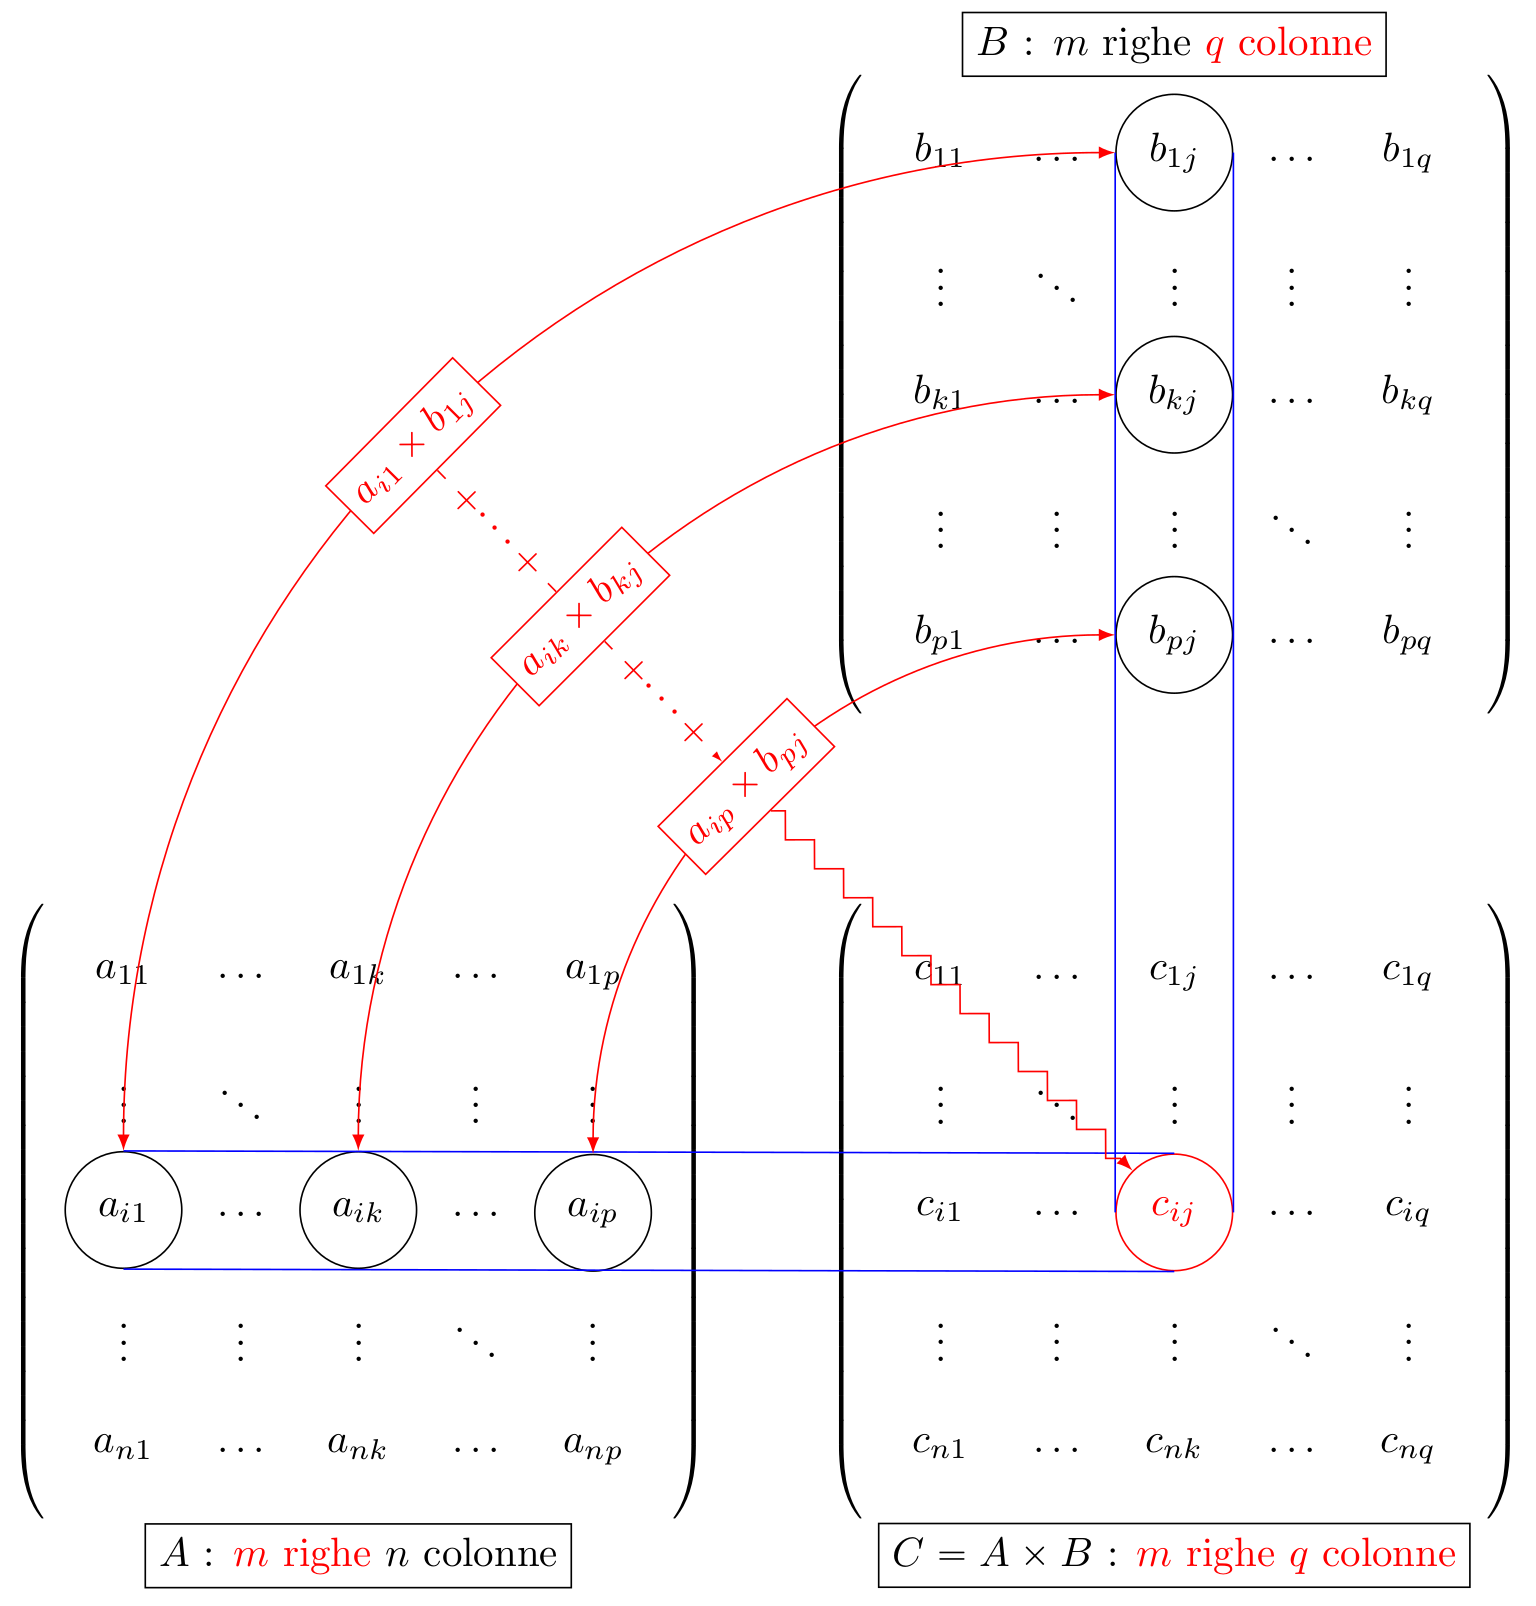
\includegraphics[width=0.6\linewidth]{images/matrMult.png}
    \caption{Illustrazione grafica per la moltiplicazione tra matrici}
    \label{fig:matrMult}
  \end{figure}
\end{Def}

\begin{SubDef}{Proprietà del prodotto tra matrici}
  Per il prodotto tra matrici vigono alcune proprietà:
  \begin{enumerate}
    \item Associativa: $(AB)C = A(BC)\quad\forall A\in\mathbb{R}^{m,n},
      B\in\mathbb{R}^{n,k},C\in\mathbb{R}^{k,q}$
      \begin{proof}
        Definiamo $D = AB\in\mathbb{R}^{m,k} = (d_{ij}) = \sum^{n}_{l=1} a_{il}b_{li}$ e
        $E = BC\in\mathbb{R}^{n,q} = (e_{ij}) = \sum^{k}_{p=1} b_{ip}c_{pi}$. Allora
        svolgiamo i calcoli
        \begin{equation*}
          (AB)C= DC = \sum^{q}_{f=1} d_{if}c_{fi} = \sum^{q}_{f=1} (a_{if}b_{fi})c_{fi}
        \end{equation*}
        e
        \begin{equation*}
          A(BC) = AE = \sum^{n}_{f=1} a_{if}c_{fi} = \sum^{q}_{f=1} a_{if}(b_{if}c_{fi})
        \end{equation*}
        Dato che $f$ va da $1$ a $q$ e che in $\mathbb{R}$ vale la proprietà associativa
        del prodotto, si può dire che
        \begin{equation*}
          \sum^{q}_{f=1} (a_{if}b_{fi})c_{fi} = \sum^{q}_{f=1} a_{if}(b_{if}c_{fi})
        \end{equation*}
      \end{proof}
    \item Distributiva del prodotto per la somma: $A(B+C) = AB+AC\quad\forall
      A\in\mathbb{R}^{m,n},B,C\in\mathbb{R}^{n,p}$
      \begin{proof}
        Per definizione di somma
        \begin{equation*}
          B+C = (b_{ij}+c_{ij})
        \end{equation*}
        Quindi
        \begin{equation*}
          A(B+C) = A(b_{ij}+c_{ij})
        \end{equation*}
        e infine
        \begin{equation*}
          A(b_{ij}+c_{ij}) = \sum^{p}_{f=1} a_{if}(b_{fi}c_{fi}) =
          \sum^{p}_{f=1} \left[ a_{if}b_{fi}+a_{if}c_{fi} \right] = \sum^{p}_{f=1}
          a_{if}b_{fi} + \sum^{p}_{f=1} a_{if}c_{fi} = AB+AC
        \end{equation*}
      \end{proof}
    \item $(\lambda A)B = \lambda(AB) = A(\lambda B)\quad\forall A\in\mathbb{R}^{m,n},
      B\in\mathbb{R}^{n,p}$
      \begin{proof}
        Per~\autoref{def:matrice_prodotto_scalare} si ha che
        \begin{equation*}
          \lambda A=(\lambda a_{ij})
        \end{equation*}
        Si ha quindi
        \begin{equation*}
          (\lambda A)B = \sum^{p}_{f=1} \lambda a_{if}b_{fi} = \overbrace{\sum^{p}_{f=1}
          a_{if}\lambda b_{fi}}^{A(\lambda B)} = \lambda \sum^{p}_{f=1} a_{if}b_{fi} =
          \lambda (AB)
        \end{equation*}
      \end{proof}
    \item Solo per le matrici quadrate: $IA = A = AI\quad\forall A\in\mathbb{R}^{n,n}$
  \end{enumerate}
\end{SubDef}
Si noti che per il prodotto $\exists A,B\suchthat AB=0 \notimplies A=O\lor B=O$. Si noti
anche che sempre per il prodotto, in generale $AB=AC\notimplies B=C$ con $A\neq O$.

\begin{Def}{Trasposto di una matrice}\label{def:matrice_trasposto}
  Data $A\in\mathbb{R}^{m,n}$ si dice trasposta di $A$ e si indica con $\transp A$ la matrice
  che si ottiene invertendo righe con colonne. Formalmente
  \begin{equation*}
    \text{Se}\; A=(a_{ij}),\; \transp A = (b_{ij})\implies b_{ij} = a_{ji}\quad\forall
    i=1,\ldots,m, j=1,\ldots,n
  \end{equation*}
\end{Def}

\begin{SubDef}{Proprietà del trasposto di una matrice}
  Il trasposto gode di alcune proprietà
  \begin{enumerate}
    \item $\transp(A+B) = \transp A+\transp B\quad\forall A,B\in\mathbb{R}^{m,n}$
    \item $\transp (\lambda A)=\lambda \transp A\quad\forall\lambda\in\mathbb{R},
      A\in\mathbb{R}^{m,n}$
    \item $\transp{(AB)} = \transp B\transp A\quad\forall A,B\in\mathbb{R}^{m,n}$
    \item Se $A\in GL(n,\mathbb{R})$ e $A^{-1}$ è la sua inversa, allora anche
      $\transp{A}\in GL(n,\mathbb{R})$ e si ha ${(\transp A)}^{-1} = \transp{(A^{-1})}$
      \begin{proof}
        Si deve dimostrare che
        \begin{equation*}
          \transp{(A^{-1})}\transp A = \transp{(AA^{-1})} = \transp I = I
        \end{equation*}
        e
        \begin{equation*}
          \transp A\transp{(A^{-1})} = \transp (A^{-1}A) = \transp I = I
        \end{equation*}
      \end{proof}
  \end{enumerate}
\end{SubDef}

\begin{Def}{Traccia di una matrice quadrata}\label{def:matrice_traccia}
  Sia $A\in\mathbb{R}^{n,n}$. Di definisce la sua traccia
  \begin{equation*}
    \tr(A)\bydef\sum_{i=1}^{n}a_{ii}
  \end{equation*}
\end{Def}

\begin{SubDef}{Proprietà della traccia}
  La traccia gode di alcune proprietà:
  \begin{enumerate}
    \item $\tr(A+B) = \tr(A) + \tr(B)\quad\forall A,B\in\mathbb{R}^{n,n}$
      \begin{proof}
        Per~\autoref{def:matrice_somma} si ha che
        \begin{equation*}
          \tr(A+B) = \sum^{n}_{i=1} (a_{ii}+b_{ii}) = \sum^{n}_{i=1} a_{ii} +
          \sum^{n}_{i=1} b_{ii} = \tr(A) + \tr(B)
        \end{equation*}
      \end{proof}
    \item $\tr(\lambda A) = \lambda\tr(A)\quad\forall\lambda\in\mathbb{R},
      A\in\mathbb{R}^{n,n}$
      \begin{proof}
        Per~\autoref{def:matrice_prodotto_scalare} si ha che
        \begin{equation*}
          \tr(\lambda A) = \sum^{n}_{i=1} \lambda a_{ii} = \lambda \sum^{n}_{i=1} a_{ii}
          = \lambda\tr(A)
        \end{equation*}
      \end{proof}
    \item $\tr(AB) = \tr(BA)\quad\forall A,B\in\mathbb{R}^{n,n}$
      \begin{proof}
        Siano $A=(a_{ij})$ e $B=(b_{ij})\in\mathbb{R}^{n,n}$. Allora $AB=(c_{ij})$. Per
        la~\autoref{def:matrice_prodotto}
        \begin{equation*}
          c_{ii} = \sum^{n}_{k=1} a_{ik}b_{ki}
        \end{equation*}
        Per la~\autoref{def:matrice_traccia}
        \begin{equation}\label{eq:matrice_traccia_3_dim_1}
          \tr(AB) = \sum^{n}_{i=1} c_{ii}= \sum^{n}_{i=1} \sum^{n}_{k=1} a_{ik}b_{ki}=
          \sum^{n}_{i,k=1} a_{ik}b_{ki}
        \end{equation}
        Sia $BA = (d_{ij})$, allora
        \begin{equation*}
          d_{ii} = \sum^{n}_{k=1} b_{ik}a_{ki}
        \end{equation*}
        Per la~\autoref{def:matrice_traccia}
        \begin{equation}\label{eq:matrice_traccia_3_dim_2}
          \tr(BA) = \sum^{n}_{i=1} d_{ii} = \sum^{n}_{i=1} \sum^{n}_{k=1} b_{ik}a_{ki} =
          \sum^{n}_{i,k=1} b_{ik}a_{ki}
        \end{equation}
        Dato che in $\mathbb{R}$ il prodotto è commutativo e che sia $i$ che $k$, sia in
        \eqref{eq:matrice_traccia_3_dim_1} e \eqref{eq:matrice_traccia_3_dim_2} variano
        da $1$ a $n$, si può affermare che
        \begin{equation*}
          \sum^{n}_{i,k=1} a_{ik}b_{ki} = \sum^{n}_{i,k} b_{ik}a_{ki}
        \end{equation*}
      \end{proof}
    \item $\tr(\transp A) = \tr(A)\quad\forall A\in\mathbb{R}^{n,n}$
      \begin{proof}
        Per~\autoref{def:matrice_trasposto} si ha che se $A$ è una matrice diagonale,
        $\transp A = A$. Dato che la traccia prende solo gli elementi sulla diagonale,
        farne il trasposto non modifica il risultato.
      \end{proof}
  \end{enumerate}
\end{SubDef}
